\documentclass[mathNotesPreamble]{subfiles}
\begin{document}
\relscale{1.4} %TODO
\section{14.1: Vector-Valued Functions}

  Vector-valued functions are functions of the form $\vecr(t)=\bracket{x(t),y(t),z(t)}$, where $x(t)$, $y(t)$, and $z(t)$ are parametric equations dependent on $t$.
  
  \begin{center}
    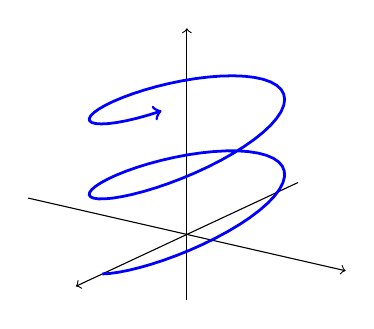
\begin{tikzpicture}
      \begin{axis}[
        axis lines=center,
        axis line style={black,->},
        xmin=-4.5, xmax=4.5,
        ymin=-2.5, ymax=2.5,
        zmin=-0.125, zmax=2,
        xmajorticks=false,
        ymajorticks=false,
        zmajorticks=false,
        enlargelimits={abs=0.75},
        view={125}{25},
        every axis plot/.append style={line width=0.5pt, color=blue}
        ]
        \addplot3[domain=0:4.25*pi, samples=100, samples y=0, ->, line width=1pt] ({4*cos(deg(x))},{sin(deg(x))},{x/6.28}); 
      \end{axis}
    \end{tikzpicture}
  \end{center}
  
  \begin{defn*}[Limit of a Vector-Valued Function]
    A vector-valued function $\vecr$ approaches the limit $\mathbf L$ as $t$ approaches $a$, written $\displaystyle\lim_{x\to a} \vecr(t)=\mathbf L$, provided $\displaystyle\lim_{x\to a}\abs{\vecr(t)-\mathbf L}=0$.
  \end{defn*}
  \pagebreak
  
\end{document}